\chapter{Cluster Analysis} \label{sec:clusteranalysis}
The problem of the cluster analysis is perhaps one of the most widely studied problems in machine learning or data mining~\cite{Aggarwal13}. It has numerous application in disciplines such as machine learning, summarization, segmentation, and target marketing~\cite{Jain10, Kaufman90}.
The basic problem of clustering may be stated as follows:\textit{Given a set of data points, find groups in data so each group consist of as similar points as possible.} This definition is very rough, because the variations in the problem definition can be significant, depending upon the specific data model used~\cite{Aggarwal13}. For example, a generative model may define similarity on the basis of probabilistic generative mechanism, whereas a distance-based approach will use a traditional distance function for the quantification. Also the data properties has a significant impact on the definition.
%In this context, objects are similar when their properties has same values or differs minimally in comparison to same property of other nearest objects or all objects in cluster. This means that each cluster contains objects that are more similar to nearest neighbors or all objects from cluster than objects from other clusters. Hence the cluster analysis may be performed only on sets of objects which must be to each other comparable - we must be able.to decide how much are two objects similar. This analysis has a wide range of applications, such as data mining, pattern recognition or machine learning.\\
\section{Definition}

Because the cluster analysis is a diverse topic, there are many underlaying algorithms, which could vary greatly. They depend on a data domain and a problem scenario~\cite{Aggarwal13}. They are also different in a cluster definition and in cluster search methods. Cluster most common definitions are following: Clusters are groups with small distances between the objects from the same cluster, dense areas of the input data, intervals, or each particular statistical distribution.\\
%If we want to define cluster analysis more precisely, it is function $f$ which groups objects $o \in O$, where $O$ is input data set and splits them into subsets. We need also the function $s$ which compares two objects and determines, how much are these objects similar $s: O \times O \to \mathbb{R}$.The task is to split items into subsets so the distances between objects from same subset are minimal. $$min \sum_{c=1}^nO_c:\sum_{i,j=1}^{|O_c|}s(o_i,o_j);o_{i,j}\in O_c;\cap_{c=1}^nO_c=O$$

Cluster analysis itself could be performed on many types of data but in this thesis, we will focus mainly on vector spaces so we could define the cluster analysis in following way:
We will take a real vector with dimension $d$ as an object, where each element of vector presents an object property. The set of vectors $V$ over field $F$ must fulfill axioms of the vector space with operations $\oplus: V \times V \to V$ called addition and $\otimes:F \times V \to V$ called multiplication:
\begin{enumerate}
\item $(\forall \vec{u}, \vec{v} \in V):\vec{u} \oplus \vec{v} = \vec{v} \oplus \vec{u}$ \textit{(addition commutativity)}
\item $(\forall \vec{u}, \vec{v}, \vec{w} \in V):(\vec{u} \oplus \vec{v}) \oplus \vec{w} = \vec{u} \oplus (\vec{v} \oplus \vec{w})$ \textit{(addition associativity)}
\item $(\exists \vec{0})(\forall \vec{v} \in V):\vec{v} \oplus \vec{0} = \vec{v}$ \textit{(identity element of addition)}
\item $(\forall \vec{u} \in V)(\exists \vec{v} \in V):\vec{u} \oplus \vec{v} = \vec{0}$ \textit{(inverse element existence)}
\item $(\forall a,b \in F)(\forall \vec{v} \in V):(a \otimes b) \otimes \vec{v} = a \otimes (b \otimes \vec{v})$ \textit{(multiplication associativity)}
\item $(\exists \textbf{1} \in F)(\forall \vec{v} \in V):\textbf{1} \otimes \vec{v} = \vec{v}$ \textit{(identity element of multiplication)}
\item $(\forall a,b \in F)(\forall \vec{v} \in V):(a + b) \otimes \vec{v} = (a \otimes \vec{v}) \oplus (b \otimes \vec{v})$ \textit{(distributivity 1)}
\item $(\forall a \in F)(\forall \vec{u}, \vec{v} \in V):a \otimes (\vec{u} \oplus \vec{v}) = (a \otimes \vec{u}) \oplus (a \otimes \vec{v})$ \textit{(distributivity 2)}
\end{enumerate}

We must also have a metric function $d:V \times V \to F$ fulfilling metric axioms:\\ \\
$ \forall  u, v, w \in V$
\begin{enumerate}
\item $d(u, v)\geq 0$ \textit{(non-negativity)}
\item $d(u, v) = 0 \iff u = v$ \textit{(identity)}
\item $d(u, v) = d(v, u)$ \textit{(symmetry)}
\item$d(u, v) \leq d(u, w) + d(w, v)$ \textit{(triangle inequality)}
\end{enumerate}

The main task is same as in common definition. We need to find a system of subsets so the distances between vectors in one subset is minimal.

\subsection{Distances}
As we mentioned in the beginning of this section, cluster analysis could be performed on many data types. This variety reflects in wide range of usable distance (or similarity) functions, because specific type of data requires specific metric. Distance function is very important to Cluster analysis because it determines very often whether a cluster analysis is applicable on concrete data type. Because in this thesis we will deal especially with vector spaces, we will start with general p-norm distance applicable on this space: $$\|a-b\|_p=\sqrt[\leftroot{-1}\uproot{3}\scriptstyle p]{\sum_i |a_i - b_i|^p} $$
Most commonly used $L_p$ distance are $L_1$ distance called \textbf{Manhattan distance} or $L_2$ distance called \textbf{Euclidian distance}.
Because computing roots is difficult, we could simplify the distance by omitting the root computation. This adjustment does not break metric axioms and it is usually called \textbf{Squared Euclidian distance}.\\

%Because all of these algorithms counts distance, appropriate metric must be used.
%\begin{description}
%\item[Manhattan distance $L_1$] $$\|a-b\|_1=\sum_i |a_i - b_i| $$
%\item[Euclidian distance $L_2$] $$\|a-b\|_2=\sqrt{\sum_i (a_i - b_i)^2 }$$
%\item[Squared Euclidian distance $L_2^2$] $$\|a-b\|_2^2=\sum_i (a_i - b_i)^2 $$
%\item[$p$-norm distance $L_p$] $$\|a-b\|_p=\Big(\sum_i |a_i - b_i|^p\Big)^\frac{1}{p} $$
%\item[Maximum distance $L_\infty$] $$\|a-b\|_\infty=\lim_{p\to\infty}\Big(\sum_i |a_i - b_i|^p\Big)^\frac{1}{p}=\max_i |a_i - b_i| $$
%\end{description}
For other input data types, we give a few examples of non vector spaces. We could take distance functions usable in statistics like \textbf{Mahalanobis distance} and \textbf{Wasserstein metric}

\subsubsection{Mahalanobis distance}
Is useful if we need to compute distances between a point $P$ and distribution $D$. The main idea of this distance is measuring ho differs $P$ from the mean of $D$.
If we have observation $p=(p_1,...,p_n)^T$ a mean of set of observations $\mu=(\mu_1,...,\mu_n)^T$ and a covariance matrix $S$, the Mahalanobis distance is defined as:
$$D_M(x) = \sqrt{(x - \mu)^T S^{-1} (x-\mu)}$$

\subsubsection{Wasserstein metric}
Another distance used in statistics is Wasserstein metric (also called Earth mover's distance (EMD))~\cite{Vallender73}. This metric is used for compute distance between two probability distributions on given metric space $M$. There is analogy with moving ``earth'' piled up in same way as shape of probability distribution. The distance is amount of ``earth'' which must be moved to change the shape of pile into another shape specified by second probability distribution times the distance it has to be moved. This distance is defined by following way:\\
Let $X$ be a metric space with metrix $\rho$ and $\mathfrak{B}$ be the $\sigma$-algebra of Borel subsets of $X$. The Wasserstein distance $R(P,Q)$ between probability distributions $P$ and $Q$ on $(X, \mathfrak{B})$ is defined as:
$$R(P,Q)=\inf\mathbf{E}\rho(\xi, \sigma)$$
where $\inf$ is taken over all possible pairs of random variables $\xi$ and $\sigma$ with distribution $P$ and $Q$.\\

There are also spaces, which are even not from mathematics but which contains objects that are also comparable.

\subsubsection{Levenshtein distance} Levenshtein distance is used for edit distance between two strings $a, b$ and it is recursively defined by following definition:
\begin{equation*}
lev_{a,b}(i,j)=
\begin{cases}
max(i,j) & $if $ min(i,j)=0, \cr
min \begin{cases}
lev_{a,b}(i-1,j) + 1 \cr
lev_{a,b}(i,j-1) + 1 \cr
lev_{a,b}(i-1,j-1) + dif(a_i,b_j)
\end{cases} & $otherwise$
\end{cases}
\end{equation*}
Where \begin{equation*}
dif(a_i,b_j)=
\begin{cases}
0 & $if $ a_i = b_j, \cr
1 & $otherwise$
\end{cases}
\end{equation*}

\subsubsection{Signature Quadratic Form Distance}
This metric becomes really useful for comparing multimedia objects, which could be described by signatures. Problem is that these signatures could differ in structure and size so we could not use distances described before. The feature of each object is described by a vector of pairs of centroid from feature space $\mathbb{FS}$ and its weight from $\mathbb{R^{+}}$.
Than we do not count distances between the feature signatures but in Signature Quadratic Form Distance~\cite{Beecks10}, the similarity functions are used.
Mathematically, Signature Quadratic Form Distance (SQFD) is defined for two feature signatures $S^{q} = \{\{c_i^q, w_i^q\}|i=1,...,n\}$ and $S^{o} = \{\{c_i^o, w_i^o\}|i=1,...,m\}$ and a similarity function $f_s(c_i,c_j) \to \mathbb{R}$ as:
$$SQFD_{f_s}(S^q,S^o)=\sqrt{(w_q|-w_o)A_{f_n}(w_q|-w_o)^T}$$
where $A_{f_n} \in \mathbb{R}^{(n+m)\times(n+m)}$ is the similarity matrix generated by applying similarity function $f_s$ to the corresponding centroids ($a_{ij}-f_s(c_i,c_j)$) and operator $|$ means concatenation of two vectors, so $w_q|-w_o = (w_1^q,...,w_n^q,-w_1^o,...,-w_m^o)$\\

Because there exists many possibilities in distance functions which covers many data types, cluster analysis has a very wide range of applicability and it is not limited by concrete data types. Because we could not cover all these possibilities in this thesis we focused on vector spaces only.

\section{Cluster Organization} \label{sec:clusterorganization}
Object organization into clusters could be done several ways depends on structure of clusters and number of clusters into which an object belongs.
\begin{description}
\item[Hard clustering] is clustering, where each object belongs to one and only one cluster. This means that hard clustering creates system where clusters are disjoint sets.
\item[Fuzzy clustering] assigns objects to clusters too, but difference is that object can belong to more than one cluster. The object membership to cluster could be specified by level or percentage of membership so object could belongs to cluster more or less based on similarity.
\item[Hierarchical clustering] is hierarchically ordered clusters creates which creates a system of subsets where the intersection of the two is either the empty set or just one of them so clusters creates structures like n-ary trees. Because of complexity of the hierarchical clustering, in this thesis we deal with non-hierarchical type only.
\end{description}
For all three types, there exists cluster version which omit isolated objects far from others called outliers. These objects are left unassigned. Because calculation with no strictly assigned objects is to complex and does not bring many advantages, in this thesis we have focused on strict clustering only.\\

There are many cluster models but in next section~\ref{sec:clustermodels}, only the best known will be described. One of the reasons why there exists a large amount of them is that the ``cluster'' cannot be precisely defined~\cite{EstivillCastro02}. Second reason is really wide applicability of this task so people from different departments approach this problem differently, because their notion of cluster differs significantly. \\

\section{Cluster Models and Algorithms} \label{sec:clustermodels}
There exist many clustering algorithms because of many cluster models. Problem is that there exist no universal algorithm, such an algorithm that covers all cluster models. Each algorithm was designed to cover one model or a subset of models and usually it is weak or not applicable for other models.

\subsection{Cluster Models}
Because there is no uniform definition of cluster, there are also many definition of cluster models. In following section, the most known models will be described.

\begin{figure}[h]
\centering
\begin{subfigure}{.49\textwidth}
  \centering
  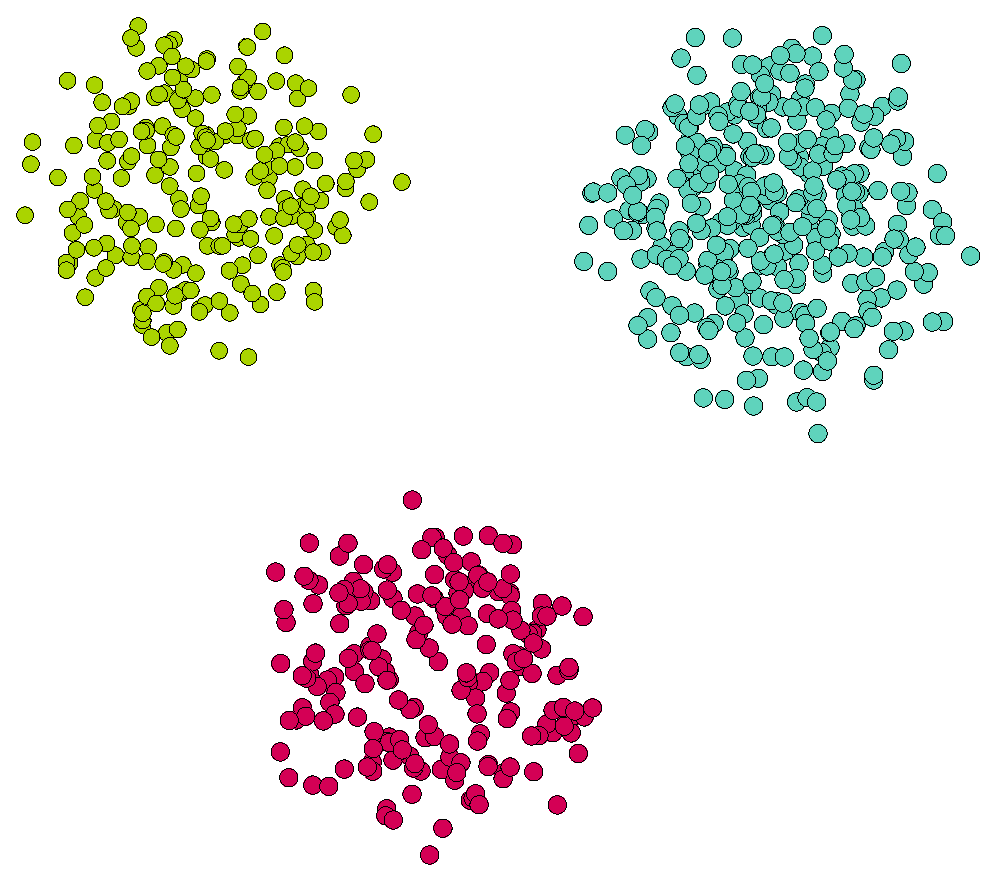
\includegraphics[width=.5\linewidth]{img/wellSeparatedObjects.eps}
  \caption{Well sepatated objects}
  \label{fig:wellSeparatedObjects}
\end{subfigure}
\begin{subfigure}{.49\textwidth}
  \centering
  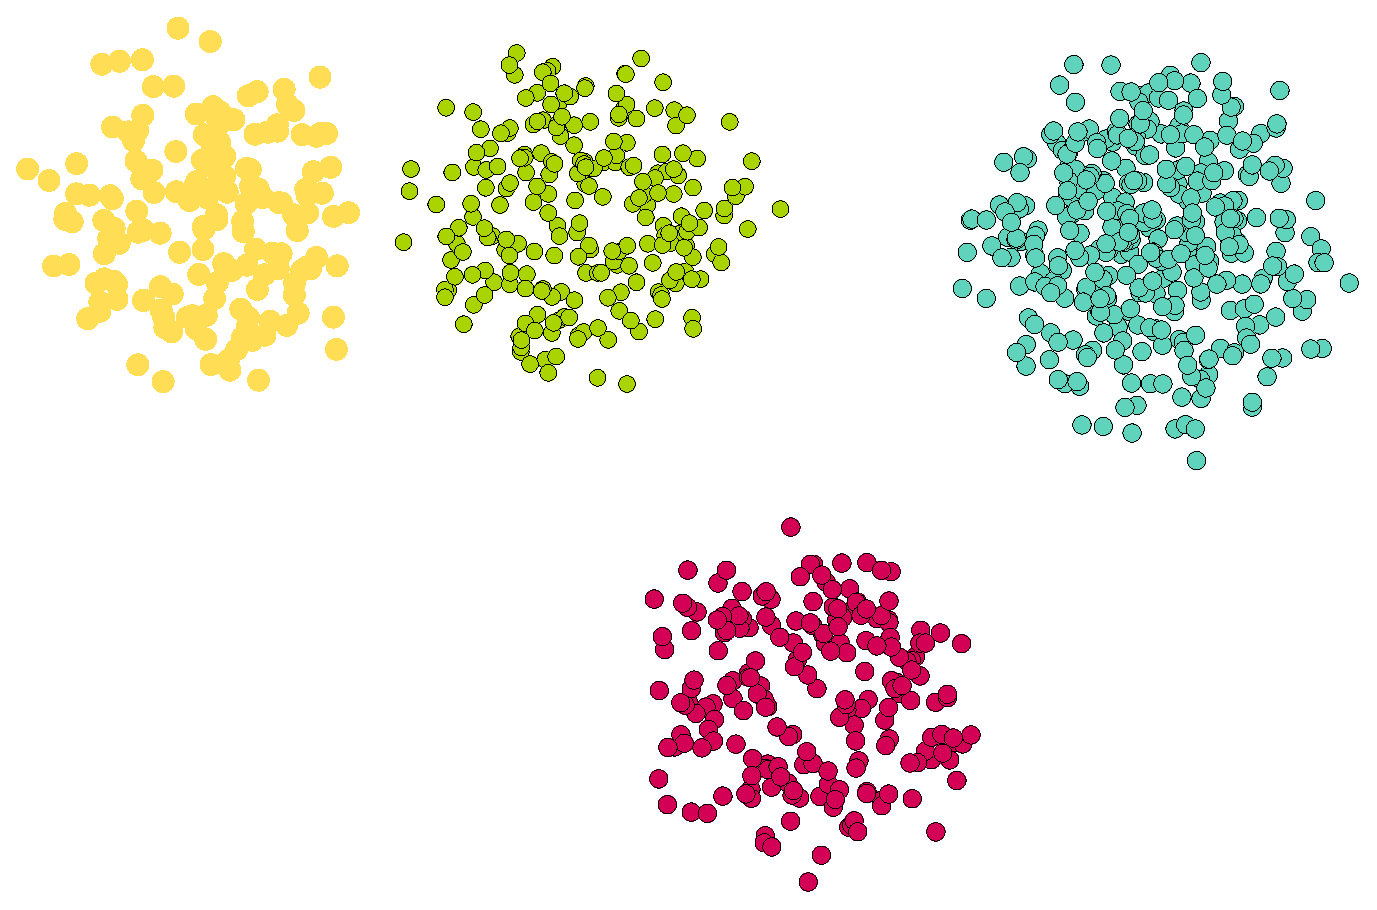
\includegraphics[width=.5\linewidth]{img/centerBasedClusters.eps}
  \caption{Center-Based Clusters}
  \label{fig:centerBasedClusters}
\end{subfigure}
\vspace*{0.5cm} 
\begin{subfigure}{.49\textwidth}
  \centering
  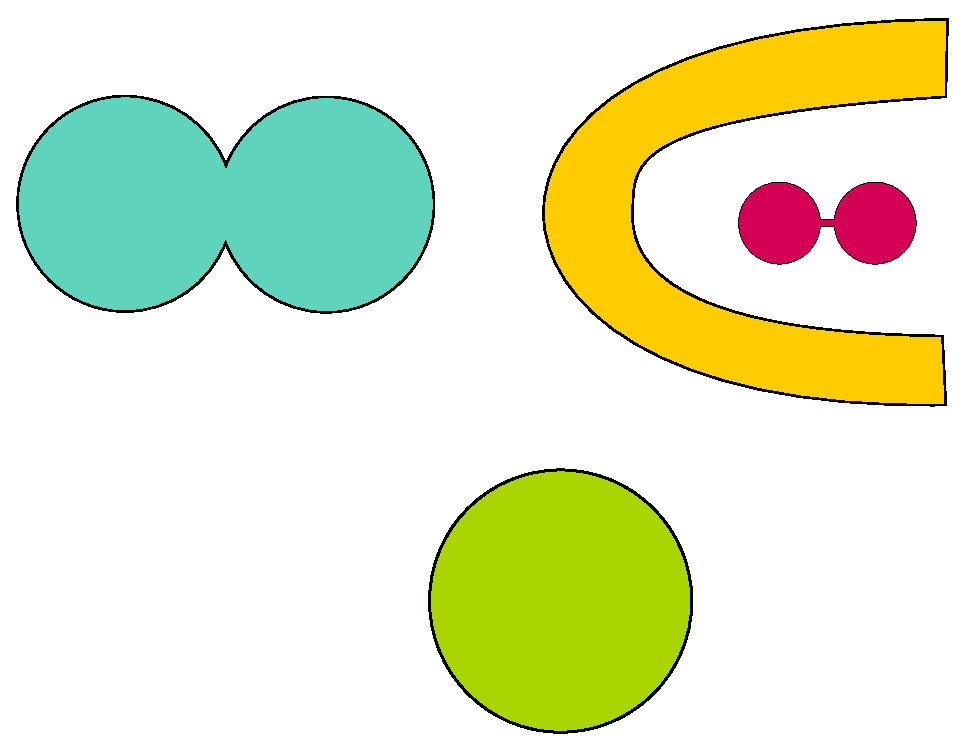
\includegraphics[width=.5\linewidth]{img/contiguousClusters.eps}
  \caption{Contiguous Clusters}
  \label{fig:contiguousClusters}
\end{subfigure}
\begin{subfigure}{.49\textwidth}
  \centering
  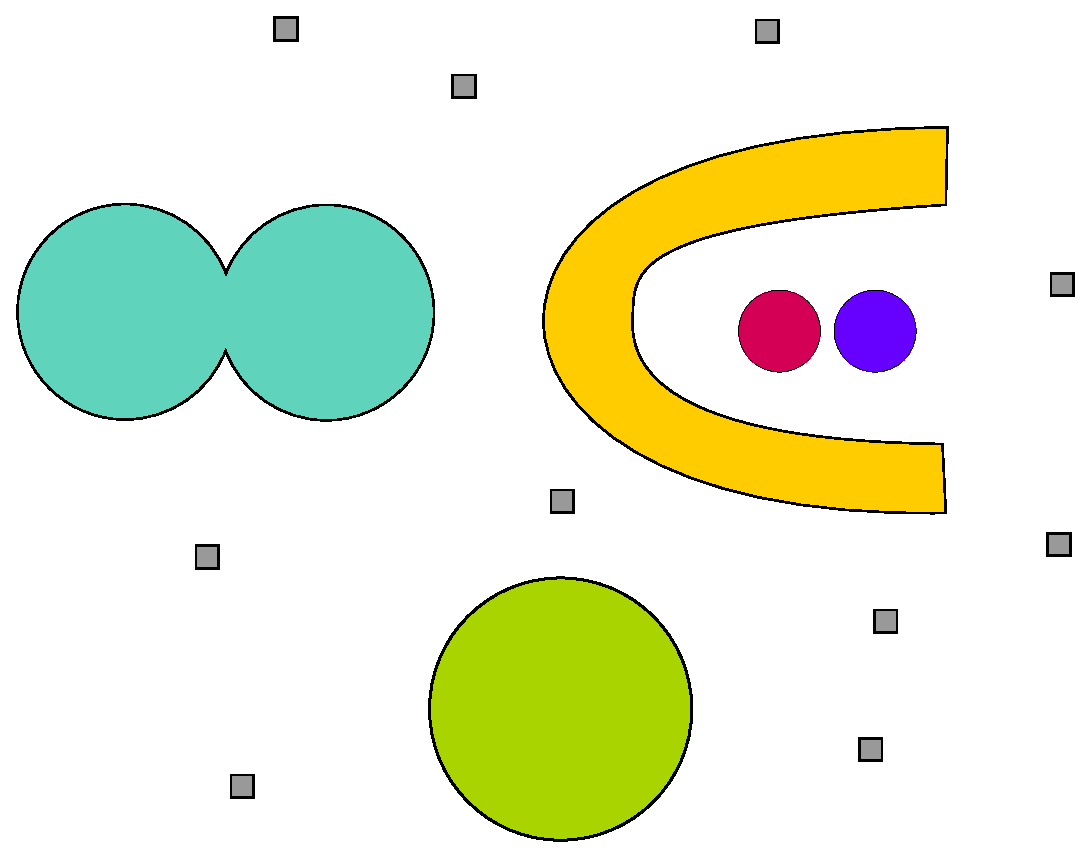
\includegraphics[width=.5\linewidth]{img/densityClusters.eps}
  \caption{Density-Based Clusters (Gray squares represent noise)}
  \label{fig:densityClusters}
\end{subfigure}
\vspace*{0.5cm} 
\begin{subfigure}{.49\textwidth}
  \centering
  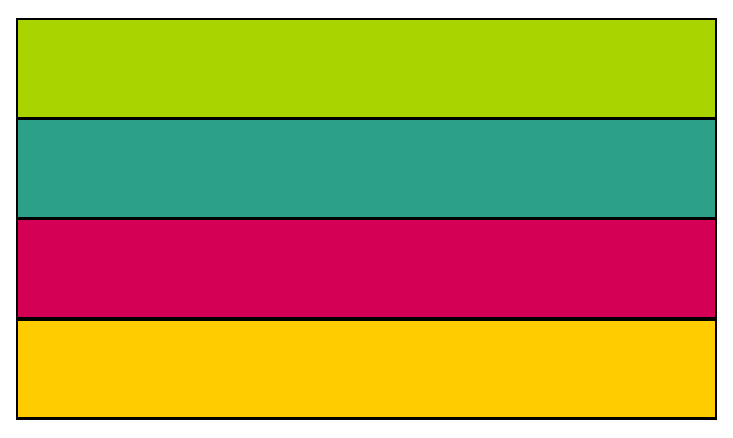
\includegraphics[width=.5\linewidth]{img/conceptualClusters.eps}
  \caption{Conceptual Clusters (Points in cluster have y-coordinate from specific range, omitting x-coordinate)}
  \label{fig:conceptualClusters}
\end{subfigure}
\begin{subfigure}{.49\textwidth}
  \centering
  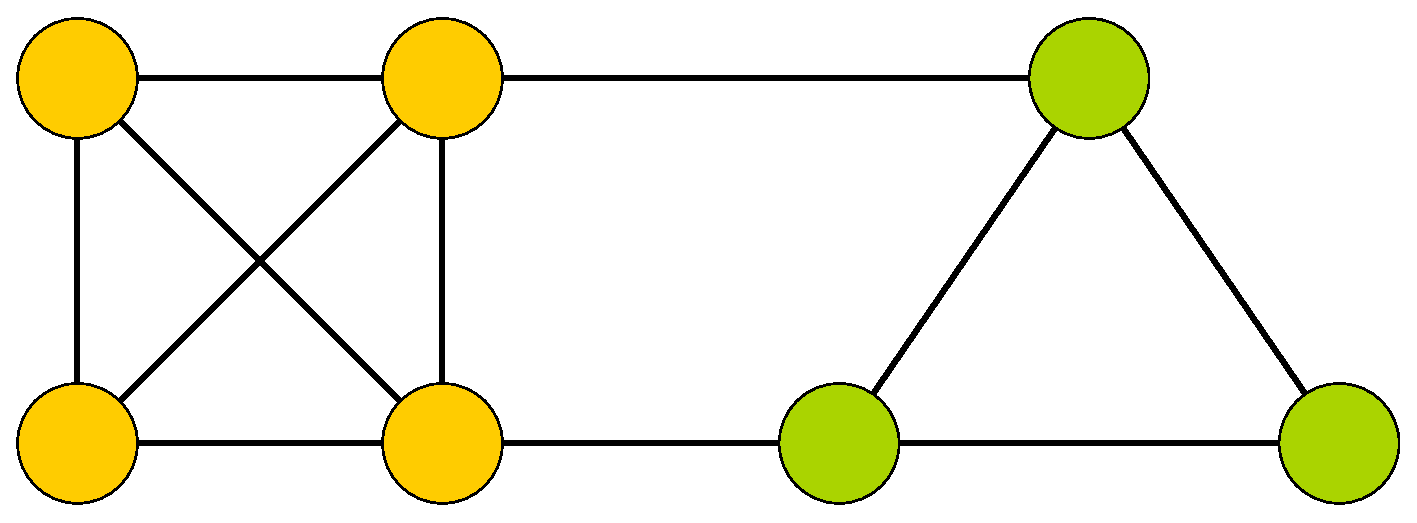
\includegraphics[width=.5\linewidth]{img/graphClusters.eps}
  \caption{Graph-Based Clusters}
  \label{fig:graphClusters}
\end{subfigure}
\caption{Typical cluster models}
\end{figure}

\begin{description}
\item[Well-Separated Clusters] Objects are easily separable-chunks of objects are not overlapping and split by sparse or empty area. Cluster is a set of objects such that each object in cluster is closer to objects from its cluster than to objects from other clusters~\autoref{fig:wellSeparatedObjects}. This is the easiest data input and most of algorithms performs well in this case.

\item[Centroid-Based Clusters] Object belongs to cluster if it is closer to the centroids of the cluster than centroids of all other clusters~\autoref{fig:centerBasedClusters}. Centroid is special object known before or precomputed. The result is similar to Voronoi space partitioning. Centroid-Based clusters are similar Voronoi cells from Voronoi diagram, where centroids are called seed or generators. This is good model for algorithms based on distance between object and centroid. \\
One of the algorithm for solving this task is \textit{\textbf{Centroid-based clustering}} representing clusters as central object, which may not be part of the input data set. This clustering is basically an optimization problem where we looking for centroids so distances will be the lowest possible. Problem is that optimization itself is NP-hard problem and the result only approximate the ideal solution. Approximation is commonly done by many iterations consist of assigning clusters to objects and counting new means.

\item[Contiguous Clusters] This model is similar to Center-Based Clusters model but there is difference that two clusters could be merged into single one if they are close enough~\autoref{fig:contiguousClusters}. In other words, object is in cluster if it is similar to one ore more other objects from cluster~\cite{Tan05}.\\
Main idea of \textbf{Contiguity-based clustering} is that objects that are nearby are more related than objects that are farther, so these algorithms grouping objects based on their distance only. Each cluster can be described by sum of distances or by maximum distance needed to connect objects in cluster. Having these cluster property, they can be easily ordered into hierarchy so parent clusters needs little more distance to connect its objects. This hierarchy could be represented as a dendrogram, which is tree diagram showing cluster hierarchy. Because this property, Contiguity-based clustering could be used for hierarchical clustering but also for hard clustering if we omit the hierarchy.\\

The connection of the objects inside cluster could be problematic. Simply, because cluster consists of many objects, there are many choices to compute the distance to. There are several methods for choosing linkage criteria between two sets of objects $A$ and $B$, $d$ is chosen metric:
\begin{description}
\item[Maximum or complete linkage clustering] $$\max\{d(a,b) : a \in A, b \in B\}$$
\item[Minimum or single linkage clustering] $$\min\{d(a,b) : a \in A, b \in B\}$$
\item[Mean or average linkage clustering, or UPGMA] (Unweighted Pair Group Method with Arithmetic Mean) $$\frac{1}{|A||B|}\sum_{a \in A} \sum_{b \in B} d(a,b)$$
\item[Centroid linkage clustering, or UPGMC] (Unweighted Pair-Group Method using Centroids) $$\|c_a - c_b\| \mbox{ where } c_a \mbox{ and } c_b \mbox{ are the centroids of clusters } A \mbox{ and } B$$
This may look like centroid based clustering but this is only a linkage criteria and the result is hierarchically ordered clusters.
\item[Minimum energy clustering] $$\frac{2}{|A||B|}\sum_{i,j=1}^{|A|,|B|}\|a_i-b_j\|_2-\frac{1}{n^2}\sum_{i,j=1}^{|A|}\|a_i-a_j\|_2-\frac{1}{|B|^2}\sum_{i,j=1}^{m}\|b_{i}-b_{j}\|_{2} : a \in A, b \in B$$
\end{description}

These methods are not resistive for extreme objects, which cause generating new clusters or even merging others. Methods has generally $O(n^3)$ complexity so they are slow for large amount of data. There exist optimization for special cases which has only complexity $O(n^2)$. These methods are taken as obsolete.

\item[Density-Based Clusters] Clusters are dense regions of objects. They are separated by low-density regions. This method is useful when some noise is present because the low-density regions will cover them and clusters will not change.~\autoref{fig:densityClusters} \\
Clusters in \textbf{Density-based clustering} are defined as areas with higher density of objects than in the rest of input data. Standalone objects are taken as noise. One of the most popular method is \textit{DBSCAN}. It is similar to contiguity-based clustering, because it connecting points based on the distance, but it only connects points satisfying density criterion. This means that in neighborhood specified by distance must be a minimum number of objects. These objects are called core objects and form the basis of cluster. Than objects which do not satisfy the density criterion but are close enough to at least one point from the cluster are added to cluster too.\\
The advantage of this method is its computational unpretentiousness, because it require only linear number of range queries. This method is deterministic so there is no need to run it in iterations.
Drawback of these methods is the $\epsilon$ density parameter so borders of clusters with smaller density could be interpreted as  noise. Also separating nearby clusters may cause problems to these methods.

\item[Distribution models] Clusters in distribution models are objects that belong to same probability distribution. It is possible that one object belongs to more clusters.\\
In \textbf{Distribution-based clustering}, clusters are defined as objects from the same or similar distribution. This approach basically emulates process of generating the input data and try to reconstruct the lost statistical parameters. Main problem of this clustering model is problem known as \textit{overfitting}. This means that more complex model is described by less complex one and the difference between them is marked as deviation or noise. For example 3 points from the neighborhood of parabola vertex will be described by linear function.\\
One of methods used in distribution-based clustering is \textit{Gaussian mixture models} where algorithm iteratively optimizing parameters of fixed number of Gaussian distributions.
Problem is that this method assuming Gaussian distributed data set, but this set may not have even a model.

\item[Conceptual Clusters] Objects in cluster has some properties same or similar, but other properties could differ significantly.~\autoref{fig:conceptualClusters}\\
As algorithm for Conceptual Clusters, we can use algorithm depends on other model properties and less significant properties of objects could be easily filtered out.

\item[Graph-Based Models] For example cliques in graphs should represent clusters. Clique is subset of nodes where every two nodes are connected with edge.~\autoref{fig:graphClusters}\\
Because of special demands of this model, special algorithms are needed so we could use graph algorithms, for example Bron-Kerbosch~\cite{Sun15} algorithm for finding cliques.
\end{description}

\subsection{K-Means} 
Clustering algorithms are wide class of algorithms and we could not focused on every clustering model and appropriate algorithm and speed it up by parallelization, because there does not exist any universal approach for speeding up but on the contrary it needs to use every single detail of the algorithm. We want to choose one of the most versatile algorithm so we decided for k-means algorithm for its wide range of usage and undemanding on the properties of the input data.\\
K-means algorithm~\cite{Aggarwal13,Tan05} is centroid based clustering algorithm. K-means input is set of $n$ points in $d$-dimensional space $R^d$, a number of output clusters $k$ and a optional number of maximum iterations $i$. \\
The task is to assign points to centroids (centers of clusters) and minimize the distance between cluster's centroid and points assigned to this cluster. Algorithm works iteratively and each iteration consist of two steps. At first step the nearest centroid is found for each point and this point is assigned to centroid's cluster. In the second step, new centroids are computed as a mean of all points assigned to same cluster. Algorithm ends after known number of steps or when nothing changes between two iterations.\\
Output of the this algorithm are centroids coordinates and points with assigned clusters.


\algdef{SE}[REPEAT]{Repat}{Until}{\algorithmicrepeat}[1]{\algorithmicuntil\ #1}

\begin{algorithm}
\caption{K-means}\label{alg:kmeans}
\begin{algorithmic}[1]
\State Select K points as the initial centroids
\Repeat
\State Make K clusters by assigning all points to the nearest cluster
\State Update centroid of each cluster
\Until{centroids do not change or maximum number of iterations reached}
\end{algorithmic}
\end{algorithm}

Because at first step we do not know the centroids, usually, the first $k$ points of input set are used as initial centroids. K-means converge fast in first few iterations, so the stopping condition could be changed to ``Until relatively few points change clusters''.~\cite{Tan05}.\\
The complexity of the computation is $O(n*k*i*d)$, where $n$ is number of input points, $k$ is number of clusters, $i$ is number of iterations and $d$ is dimension of space.\\

To evaluate k-means output, we need to somehow measure the quality of cluster assignment. For this purpose is most commonly used \textbf{Sum of Squared Error (SSE)} function. Single point error is represented by distance from the centroid of assigned cluster and the function than sums square errors of all points.
$$SSE = \sum^k_{i=1}\sum_{o \in O_i}|o,c_i|^2, \textrm{ $c_i$ \textit{is centroid of cluster} $O_i$ }$$
If we had results with bad $SSE$, we could reduce it by increasing number of clusters $k$, but this may not help if initial clusters are chosen badly.

The initial centroids are one of the disadvantages of k-means algorithm because we need to know the number of output clusters at the beginning and after computation start this number could not be changed. This possibility might be demanded by some type of problems and k-means is inconvenient for them. In addition to that, problem is also selecting of initial centroids. Although we choose ideal $k$ for the input data, the probability we chose objects from different clusters as initial points is really small~\cite{Tan05}: $$P = \frac{\mbox{number of ways to select one centroid from each cluster}}{\mbox{number of ways to select K centroids}}=\frac{k!{n \choose k}}{k^k {n \choose k} }=\frac{k!}{k^k}$$ This probability is close to zero even for small $k$, for example for $k=10$, probability is $0.00036$.\\
There are some ways to solve this problem and pickup better initial points~\cite{Tan05}:
\begin{description}
\item[multiple runs] k-means algorithm is run multiple times with different initial centroid and the best one is chosen.
\item[samples] Sample input data with hierarchical clustering and determine initial centroids.
\item[more centroids] Select more than $k$ centroids and then selects the most widely separated ones.
\item[postprocessing] Result of the algorithm is postprocessed - Clusters with high $SSE$ could be split and on the other side close clusters with low $SSE$ could be merged.
\end{description} 

Other problem of k-means is that the basic version could produce empty clusters. This could be solved by algorithm update: when we found empty cluster, we could choose point which contributes most to $SSE$ as centroid instead of empty cluster or we can choose point from the cluster with greatest $SSE$~\cite{Tan05}.

Also if clusters differs significantly in size/density/non-globular shapes~\cite{Tan05}, cluster analysis could be problem for k-means\\
For example, because the main goal of k-means is to produce similar sized clusters, we will have problem with input data where one big cluster contains many objects and one smaller cluster has only few objects~\autoref{fig:kmeansbadinputsize}. Than k-means divide the bigger cluster~\autoref{fig:kmeansbadoutputsize} so some objects from bigger that are closer centroid to smaller cluster are assigned to smaller cluster which could be undesirable because k-means ignores input data distribution.
\begin{figure}[h]
\centering
\begin{subfigure}{.49\textwidth}
  \centering
  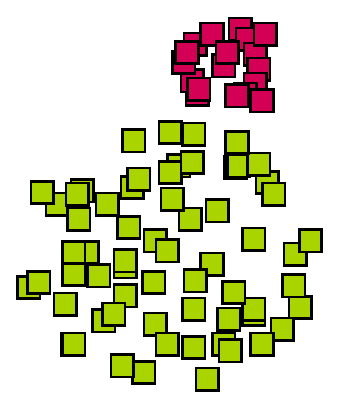
\includegraphics[width=.5\linewidth]{img/kmeans_badInputSampleSize.eps}
  \caption{Input data (assigned to clusters only for demonstration)}
  \label{fig:kmeansbadinputsize}
\end{subfigure}
\begin{subfigure}{.49\textwidth}
  \centering
  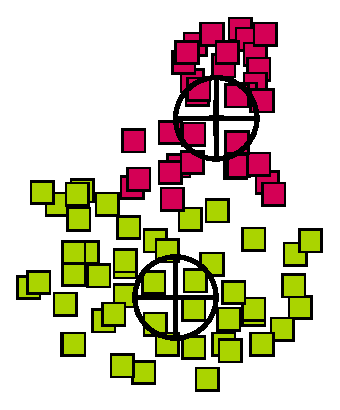
\includegraphics[width=.5\linewidth]{img/kmeans_badOutputSampleSize.eps}
  \caption{k-means output}
  \label{fig:kmeansbadoutputsize}
\end{subfigure}
\caption{K-means bad sized samples}
\end{figure}

Next problem is caused by cluster density. When we have some close dense clusters and cluster signle sparse cluster~\autoref{fig:kmeansbadinputdensity}, k-means usually mark dense clusters as one and split sparse cluster into multiple clusters.~\autoref{fig:kmeansbadoutputdensity}
\begin{figure}[h]
\begin{subfigure}{.49\textwidth}
  \centering
  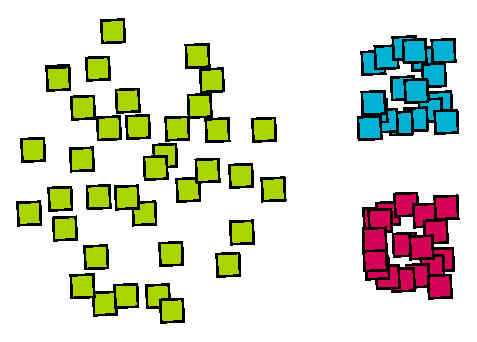
\includegraphics[width=.5\linewidth]{img/kmeans_badInputSampleDensity.eps}
  \caption{Input data (assigned to clusters only for demonstration)}
  \label{fig:kmeansbadinputdensity}
\end{subfigure}
\begin{subfigure}{.49\textwidth}
  \centering
  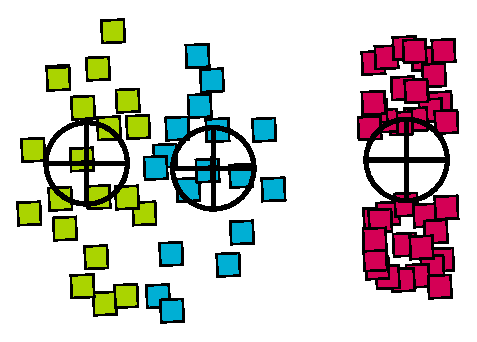
\includegraphics[width=.5\linewidth]{img/kmeans_badOutputSampleDensity.eps}
  \caption{k-means output}
  \label{fig:kmeansbadoutputdensity}
\end{subfigure}
\caption{K-means bad density clusters}
\end{figure}

Other problem is that k-means algorithm does not recognize cluster shape and produce only globular clusters. This could be problem when two usually non-convex clusters~\autoref{fig:kmeansbadinputshape} are close enough and one interferes into convex hull of the other. Than, k-means usually assigns points from one cluster to another and vice versa~\autoref{fig:kmeansbadoutputshape}.
\begin{figure}[h]
\begin{subfigure}{.49\textwidth}
  \centering
  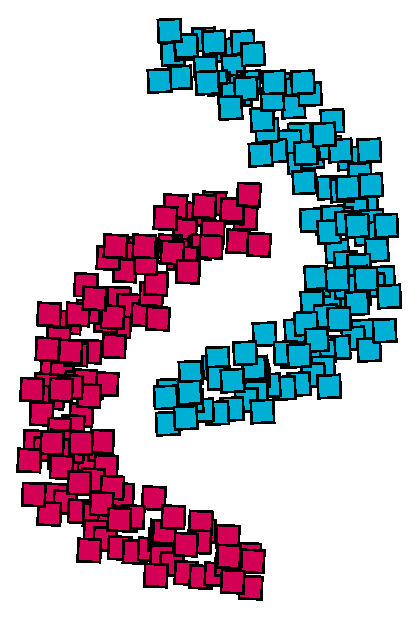
\includegraphics[width=.5\linewidth]{img/kmeans_badInputSampleShape.eps}
  \caption{Input data (assigned to clusters only for demonstration)}
  \label{fig:kmeansbadinputshape}
\end{subfigure}
\begin{subfigure}{.49\textwidth}
  \centering
  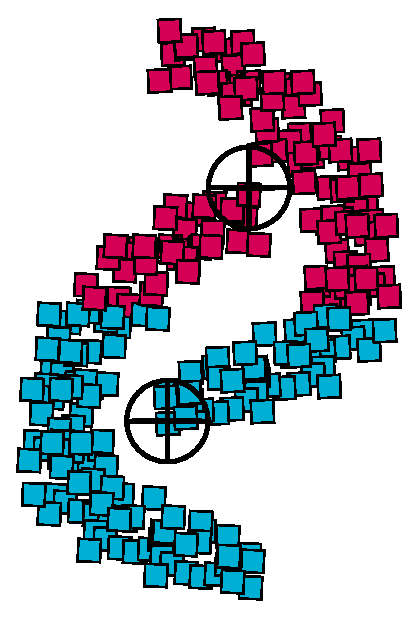
\includegraphics[width=.5\linewidth]{img/kmeans_badOutputSampleShape.eps}
  \caption{k-means output}
  \label{fig:kmeansbadoutputshape}
\end{subfigure}
\caption{K-means non-globular clusters}
\end{figure}

These problems could be solved by using more clusters than input data naturally requires. For example, input data~\autoref{fig:kmeansbadinputshape} contains two natural clusters, but when we try to split data into more clusters, the result will contain small clusters which contain only points from single original cluster and not from the other one~\autoref{fig:kmeansbadoutputsolution}. If we post process this data, we could get expected result and prevent this k-means deficiency.
\begin{figure}[h]
  \centering
  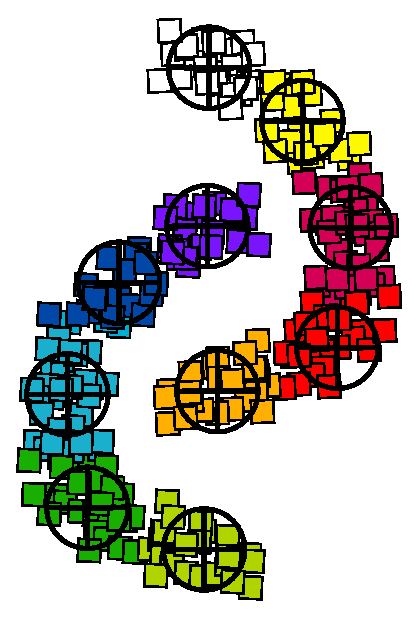
\includegraphics[width=.3\textwidth]{img/kmeans_badOutputSampleShapeSolution.eps}
  \caption{K-means solution for bad shaped cluster}
  \label{fig:kmeansbadoutputsolution}
\end{figure}


\subsubsection{K-Means Variants}
Because k-means is universal algorithm, there exists some variants if classical k-means algorithm is inconvenient or unusable. These variants could solve some problems and limitations of classical k-means algorithm.
\begin{description}
\item[k-medoids] - centroids are not virtual points in $R^d$ space but point from input data whose average dissimilarity to all other objects in cluster is minimal (medoid is used instead of mean).
\item[k-medians] - same algorithm as k-means, but in each dimension, median is used instead of mean for computing new centroid.
\item[k-means++] - initial centers are chosen randomly. This selection avoid bad inputs.
\item[Fuzzy C-means] - fuzzy cluster~\ref{sec:clusterorganization} assignment is allowed. Object does not belong strictly to one centroid but it has degree of belonging to cluster. The weighted mean (with the degree of belonging as weight) is used for computation new centroids.
\item[Bisecting k-means]~\cite{Tan05} is variant of k-means, which produce hierarchical clustering.It works also iteratively as k-means, but in each step, the clusters with highest SSE is bisected by classical k-means algorithm with $k=2$. The algorithm iterates until it reaches the number of needed clusters.~\autoref{alg:bisectingkmeans}
\begin{algorithm}
\caption{Bisecting k-means}\label{alg:bisectingkmeans}
\begin{algorithmic}[1]
\State Insert all points into the list of clusters as single cluster
\Repeat
\State Select first cluster from the list of clusters
\For{i=1 to number of iterations}
\State Bisect selected cluster using k-means algorithm
\EndFor
\State Add the two clusters from the bisection with the lowest SSE to the list of the clusters
\State Update centroid of each cluster
\Until{list of clusters contains k clusters}
\end{algorithmic}
\end{algorithm}

\end{description}
